\documentclass[11pt,a4paper]{article}

\usepackage[margin=2.3cm]{geometry}
\usepackage{amsmath,amssymb}
\usepackage{graphicx}
\usepackage{booktabs}
\usepackage{xcolor}
\usepackage{enumitem}
\usepackage[hidelinks]{hyperref}
\usepackage{caption}

\emergencystretch=1.5em
\captionsetup{font=small,labelfont=bf,width=.92\textwidth}
\setlength{\parskip}{4pt plus 1pt}
\setlength{\parindent}{0pt}

\newcommand{\code}[1]{\texttt{#1}}
\newcommand{\bst}[1]{\textbf{#1}}
\newcommand{\Kp}{K'}

\title{Top-$(K{+}J)$ with the RBLapSum surrogate versus hard Top-$\Kp$\\[2pt]
\large Research note: what the candidate window buys}
\author{}
\date{2026-09-22.}

\begin{document}
\maketitle
\vspace{-2em}

% ============================================================
\section{Purpose and summary of conclusions}
% ============================================================

The RBLapSum \code{through\_rank\_kappa} bottleneck keeps $K$ features in the
forward pass and gives gradient to a candidate pool of $K+J$. A hard Top-$\Kp$
bottleneck with $\Kp = K+J$ keeps the whole pool. The two therefore see the
same number of candidate features, but the surrogate model activates fewer of
them: $J$ enters only the backward pass, and inference skips the surrogate
machinery entirely.

This note asks what the candidate window is worth. Two questions are
separable:

\begin{itemize}[leftmargin=1.4em]
\item at a fixed \emph{candidate pool} $\Kp = K+J$, does the surrogate with $K$
active features reach the loss of hard Top-$\Kp$, which activates all $\Kp$?
\item at a fixed \emph{active count} $K$, how much does widening $J$ help?
\end{itemize}

Both variants identified in the stabilization note are included, since the
better one was configuration-dependent there: $T=2$, and an RMSNorm on each
bottleneck's output at $T=1$ (``post-norm''). All hard baselines carry the
post-norm as well.

The main conclusions are:

\begin{itemize}[leftmargin=1.4em]
\item \textbf{With the post-norm, a pool twice the active count beats hard
Top-$\Kp$ outright, at every scale tested.} For $J=K$ -- that is,
$\Kp = 2K$ -- the surrogate model wins in all four pools, by $0.009$ to
$0.014$ nats, while activating half as many features:
$1.5310$ vs $1.5408$ at $\Kp{=}64$, $1.4834$ vs $1.4938$ at $\Kp{=}128$,
$1.4423$ vs $1.4560$ at $\Kp{=}256$, and $1.4146$ vs $1.4232$ at
$\Kp{=}512$.

\item \textbf{The best configuration in the comparison is $K=256$, $J=256$
with the post-norm}, at $1.4146$: better than hard Top-512 ($1.4232$) with
half the active features, and better than hard Top-256 ($1.4560$) by
$0.041$ nats at the same active count.

\item \textbf{At a matched active count the surrogate is worth $0.04$--$0.11$
nats}, and the margin shrinks as $K$ grows: $0.107$ at $K=32$, $0.087$ at
$K=64$, $0.064$ at $K=128$, $0.041$ at $K=256$.

\item \textbf{Widening $J$ helps monotonically, except at the extreme.} At
$K=64$, $128$ and $256$ every increase in $J$ improves the loss. At $K=32$
the improvement stops and reverses at $J=480$: post-norm goes $1.5310 \to
1.5115 \to 1.4949$ for $J=32,96,224$ and then back to $1.5370$ at $J=480$.

\item \textbf{$T=2$ never reaches hard Top-$\Kp$}, trailing the matched hard
baseline by $0.008$--$0.024$ nats in all four pools, and it is worse than the
post-norm in 8 of the 10 cells. The two exceptions are both at $K=32$ with
the widest windows ($J=224$ and $J=480$), which is also where the post-norm
is weakest -- the same configuration dependence the stabilization note
found.

\item \textbf{No run diverged}, including both $K=256$ cells, which the
initialization screening had flagged as the most likely to fail.
\end{itemize}

% ============================================================
\section{Setup}
% ============================================================

Twenty-five cells, all under full magnitude--direction decoupling with the
architecture, data, optimizer, schedules and seed of the earlier campaigns
(8$\times$768, \code{abs\_topk} over $N=1536$ features, \code{residual\_out}
placement, batch $96\times512$ tokens, 20k steps, $b_0=0$).

The grid is $K, \Kp \in \{32, 64, 128, 256, 512\}$ with $J = \Kp - K > 0$,
which gives ten $(K,\Kp)$ pairs; $\Kp = 32$ has no partner because the $K$
grid starts there. Each pair was trained under both variants, and each
$\Kp$ has a hard Top-$\Kp$ baseline with the post-norm:

\begin{center}\small
\begin{tabular}{lll}
\toprule
arm & kernel / normalization & active features \\
\midrule
$T=2$              & $T=2$, no output norm        & $K$ \\
post-norm          & $T=1$, RMSNorm per bottleneck output & $K$ \\
hard Top-$\Kp$     & no surrogate, RMSNorm per bottleneck output & $\Kp$ \\
\bottomrule
\end{tabular}
\end{center}

Eleven runs were trained for this note: the $K=256$, $J=256$ cell in both
variants; the post-norm cells at $(32,96)$, $(32,224)$ and $(64,192)$; the
same three cells re-run at $T=2$ with $b_0 = 0$, replacing older $b_0 = 0.1$
runs; and hard Top-$\Kp$ with post-norm at $\Kp = 64$, $128$ and $256$. The
remaining fourteen cells are the matching arms of the stabilization campaign
and the two hard post-norm runs from the preceding note. Every cell used in
the tables below is therefore a $b_0 = 0$ run; where a cell had been trained
more than once, the selection order is stabilization campaign, then this
campaign, then the kappa ablation, and \code{scripts/plot\_kj\_comparison.py}
prints the run backing each cell.

One asymmetry is worth keeping in view when reading the tables. The candidate
window costs nothing at inference: \code{hard\_inference} skips the surrogate,
so a trained model's forward pass depends on $K$ and not on $J$. Within the
bottleneck the encoder projection is dense in $N$ regardless, while the
decoder reads a $K$-sparse code, so the $K$-dependent part of the cost is
roughly proportional to $K$. A cell that matches hard Top-$\Kp$ at $K < \Kp$
is thus the cheaper model at equal quality.

% ============================================================
\section{Results}
% ============================================================

Final validation CE after 20k steps. Rows are the active count $K$, columns
the candidate pool $\Kp = K+J$, and the last row is hard Top-$\Kp$ with the
post-norm. Bold marks the cells that beat the hard baseline in their own
column.

\begin{center}\small
\textbf{$T=2$}\\[2pt]
\begin{tabular}{lcccc}
\toprule
$K$ & $\Kp{=}64$ & $\Kp{=}128$ & $\Kp{=}256$ & $\Kp{=}512$ \\
\midrule
$32$   & 1.5492 & 1.5146 & 1.4842 & 1.4943 \\
$64$   & ---    & 1.5142 & 1.4922 & 1.4727 \\
$128$  & ---    & ---    & 1.4802 & 1.4598 \\
$256$  & ---    & ---    & ---    & 1.4425 \\
\midrule
hard Top-$\Kp$ & 1.5408 & 1.4938 & 1.4560 & 1.4232 \\
\bottomrule
\end{tabular}
\end{center}

\begin{center}\small
\textbf{post-norm}\\[2pt]
\begin{tabular}{lcccc}
\toprule
$K$ & $\Kp{=}64$ & $\Kp{=}128$ & $\Kp{=}256$ & $\Kp{=}512$ \\
\midrule
$32$   & \bst{1.5310} & 1.5115 & 1.4949 & 1.5370 \\
$64$   & ---    & \bst{1.4834} & 1.4602 & 1.4538 \\
$128$  & ---    & ---    & \bst{1.4423} & 1.4294 \\
$256$  & ---    & ---    & ---    & \bst{1.4146} \\
\midrule
hard Top-$\Kp$ & 1.5408 & 1.4938 & 1.4560 & 1.4232 \\
\bottomrule
\end{tabular}
\end{center}

The bold entries are exactly the diagonal $J=K$. Under the post-norm every
pool is won by its $K = \Kp/2$ cell and by no other: at $\Kp = 512$, for
instance, $K=256$ wins by $0.0086$, $K=128$ trails by $0.0062$, $K=64$ by
$0.031$ and $K=32$ by $0.114$. Under $T=2$ no cell wins any pool.

\paragraph{At a matched active count.}
Read along a row instead, against the hard baseline with the \emph{same}
active count:

\begin{center}\small
\begin{tabular}{lccc}
\toprule
$K$ & best post-norm cell & hard Top-$K$ & difference \\
\midrule
$32$  & 1.4949 ($J=224$) & 1.6022 & $-0.1073$ \\
$64$  & 1.4538 ($J=448$) & 1.5408 & $-0.0870$ \\
$128$ & 1.4294 ($J=384$) & 1.4938 & $-0.0644$ \\
$256$ & 1.4146 ($J=256$) & 1.4560 & $-0.0414$ \\
\bottomrule
\end{tabular}
\end{center}

The surrogate is worth between $0.04$ and $0.11$ nats at fixed activation
cost, and the margin narrows steadily with $K$ -- consistent with the
candidate window mattering most when the forward support is most restrictive.

\paragraph{The effect of widening $J$.}
At fixed $K$, with the post-norm:

\begin{center}\small
\begin{tabular}{llllll}
\toprule
$K$ & \multicolumn{4}{c}{final validation CE by $J$} & trend \\
\midrule
$32$  & $J{=}32$: 1.5310 & $J{=}96$: 1.5115 & $J{=}224$: 1.4949 & $J{=}480$: 1.5370 & reverses \\
$64$  & $J{=}64$: 1.4834 & $J{=}192$: 1.4602 & $J{=}448$: 1.4538 & & monotone \\
$128$ & $J{=}128$: 1.4423 & $J{=}384$: 1.4294 & & & monotone \\
$256$ & $J{=}256$: 1.4146 & & & & --- \\
\bottomrule
\end{tabular}
\end{center}

The reversal at $K=32$, $J=480$ is a window fifteen times the active count,
and it is the one cell where $T=2$ clearly beats the post-norm ($1.4943$
against $1.5370$). Both facts point the same way: a very wide window relative
to $K$ is the regime where the surrogate's boundary term is hardest to
control, and where the kernel width rather than the output norm is the
effective remedy.

\subsection*{Per candidate pool}

Each figure fixes the pool $\Kp = K+J$ and compares hard Top-$\Kp$ (dashed,
black) with every surrogate cell sharing that pool (solid, a blue ramp running
light to dark with increasing $J$). Left column $T=2$, right column post-norm;
the lower row repeats both panels with the vertical axis capped at 2.0 nats.

\begin{figure}[p]\centering
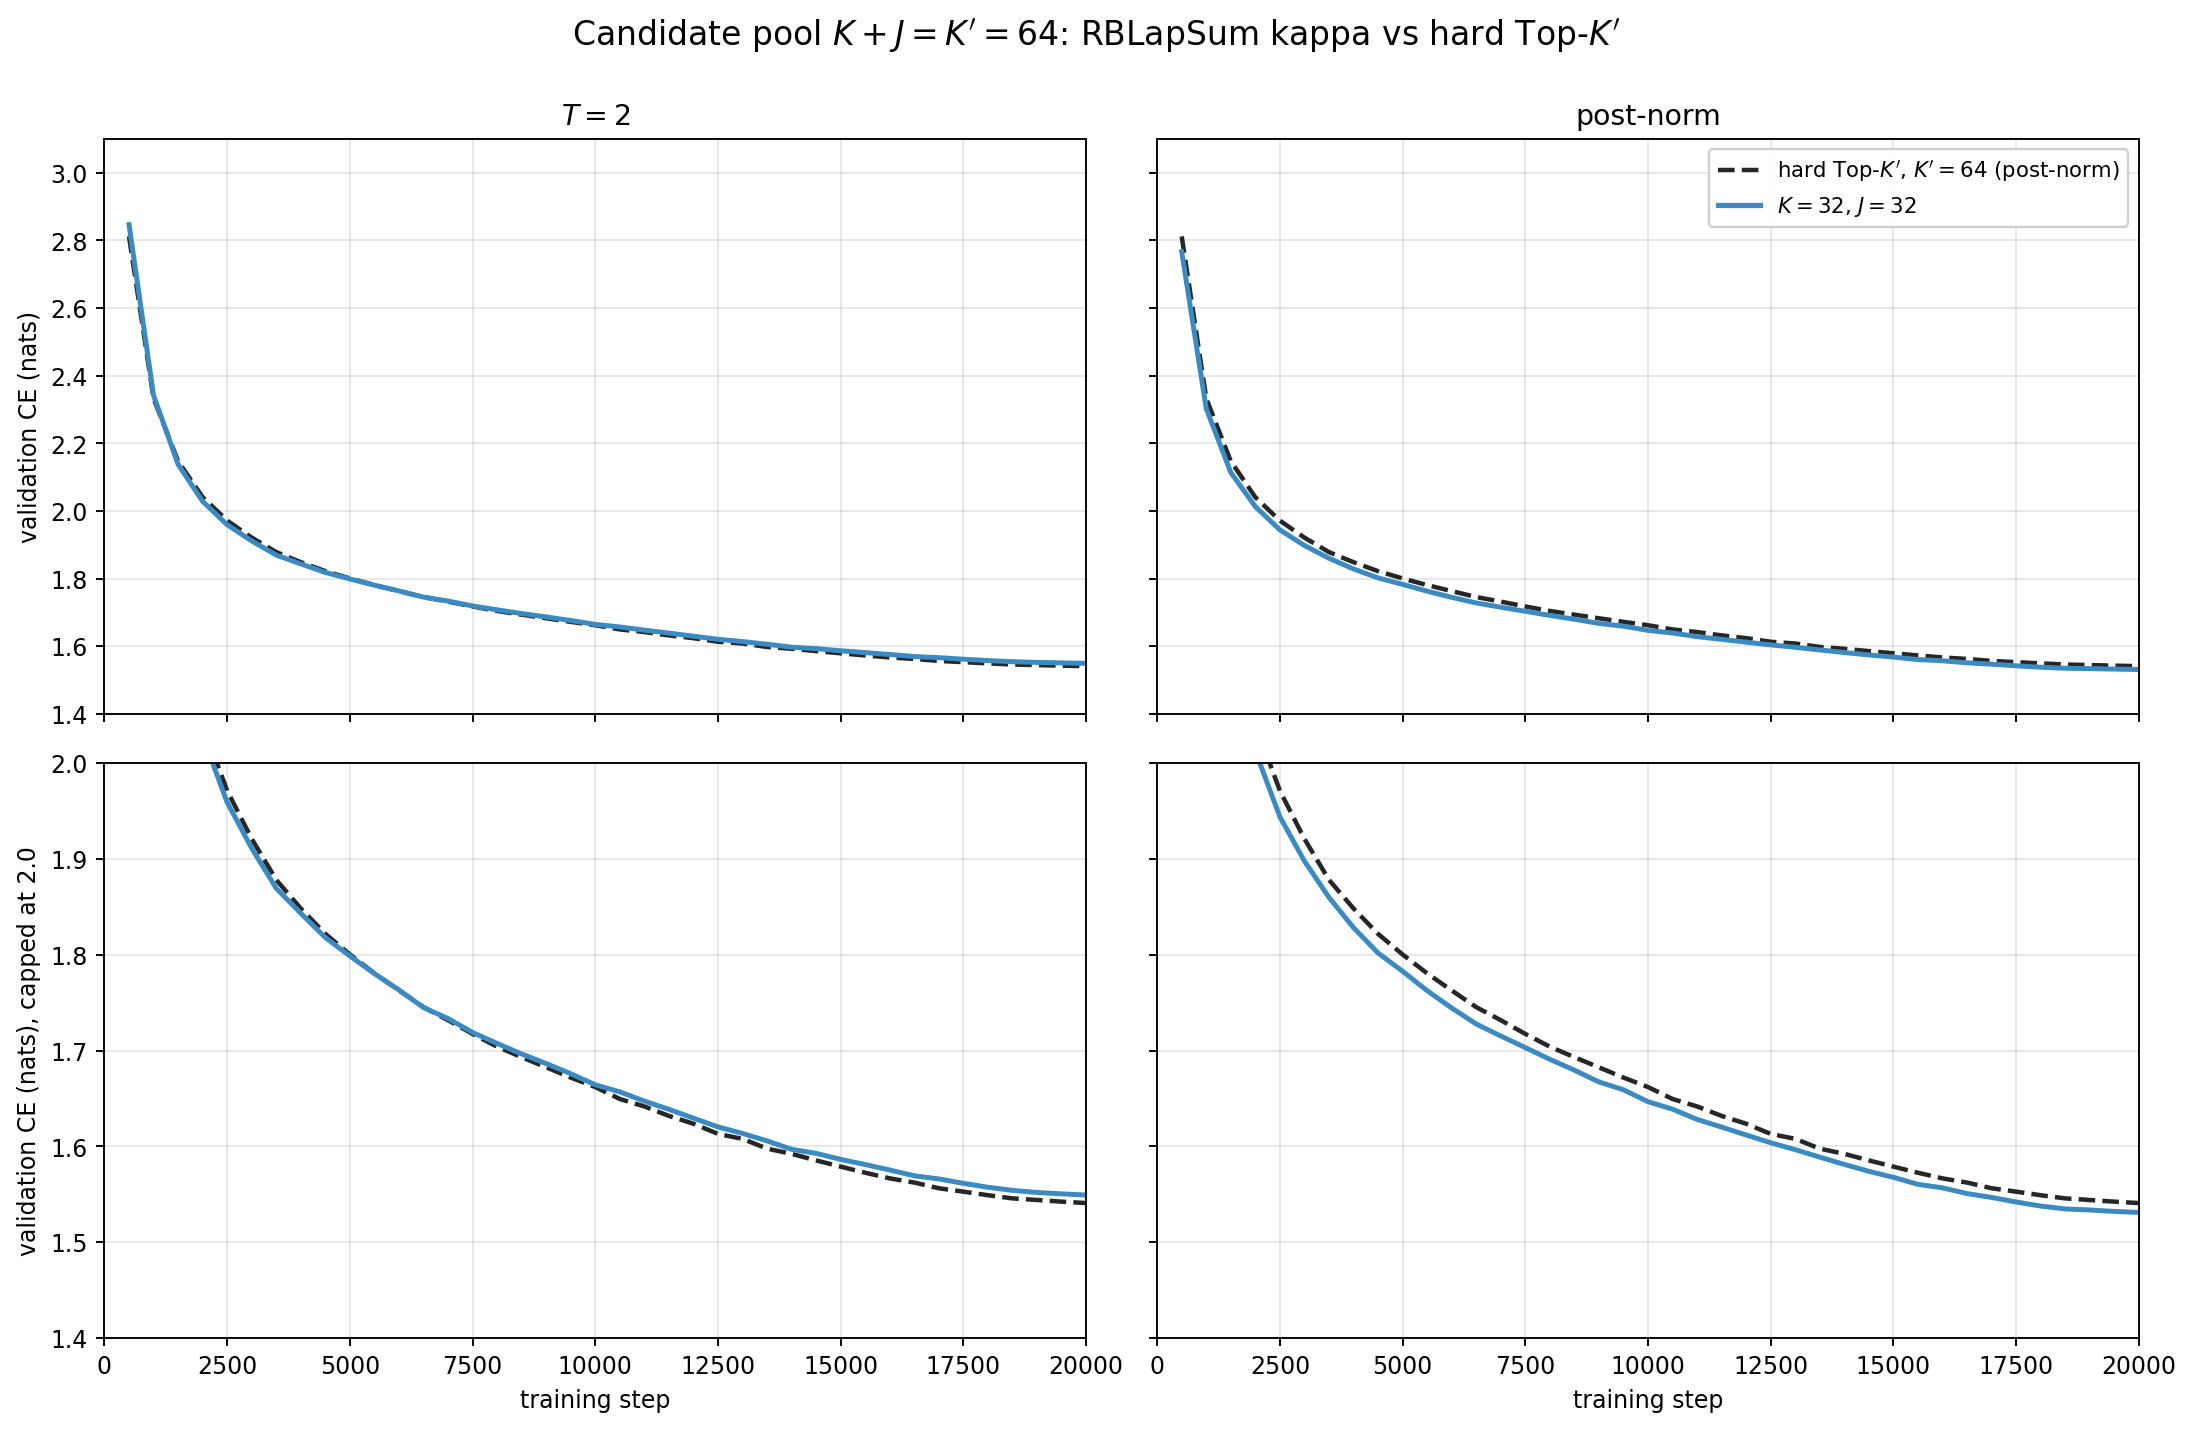
\includegraphics[width=\textwidth]{figures/kj_pool_k64.png}
\caption{$\Kp = 64$. The single surrogate cell ($K=32$, $J=32$) ends below
hard Top-64 under the post-norm and slightly above it at $T=2$.}
\end{figure}

\begin{figure}[p]\centering
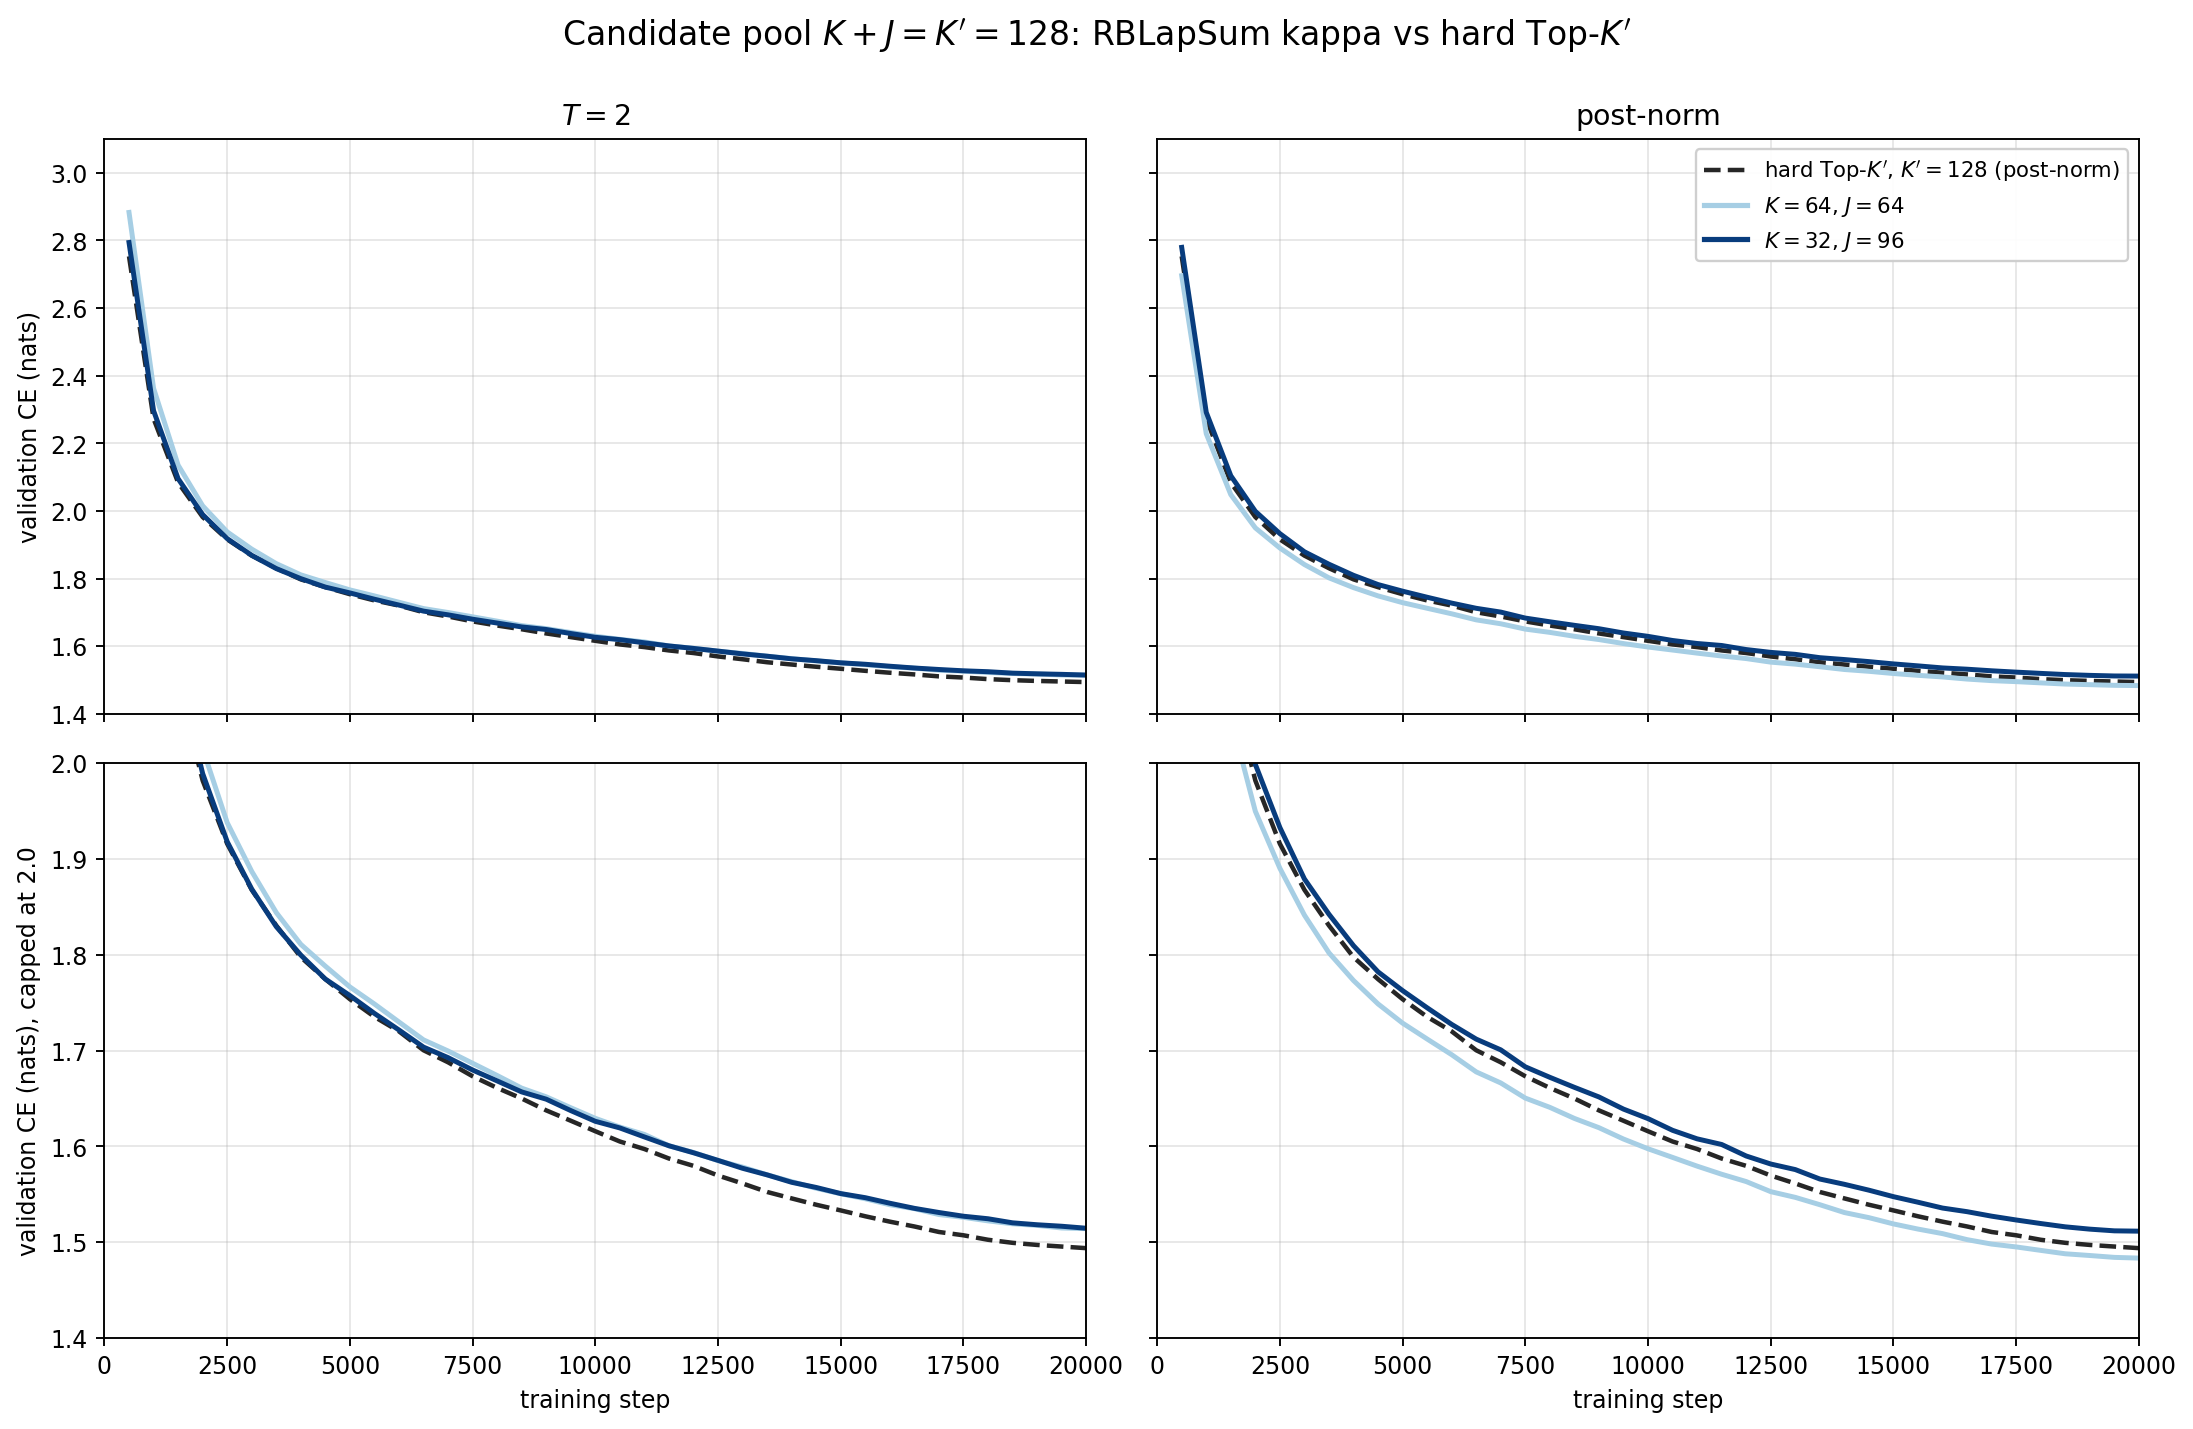
\includegraphics[width=\textwidth]{figures/kj_pool_k128.png}
\caption{$\Kp = 128$. $K=64$ wins the pool under the post-norm; $K=32$, with
the same pool but half the active count, trails the hard baseline.}
\end{figure}

\begin{figure}[p]\centering
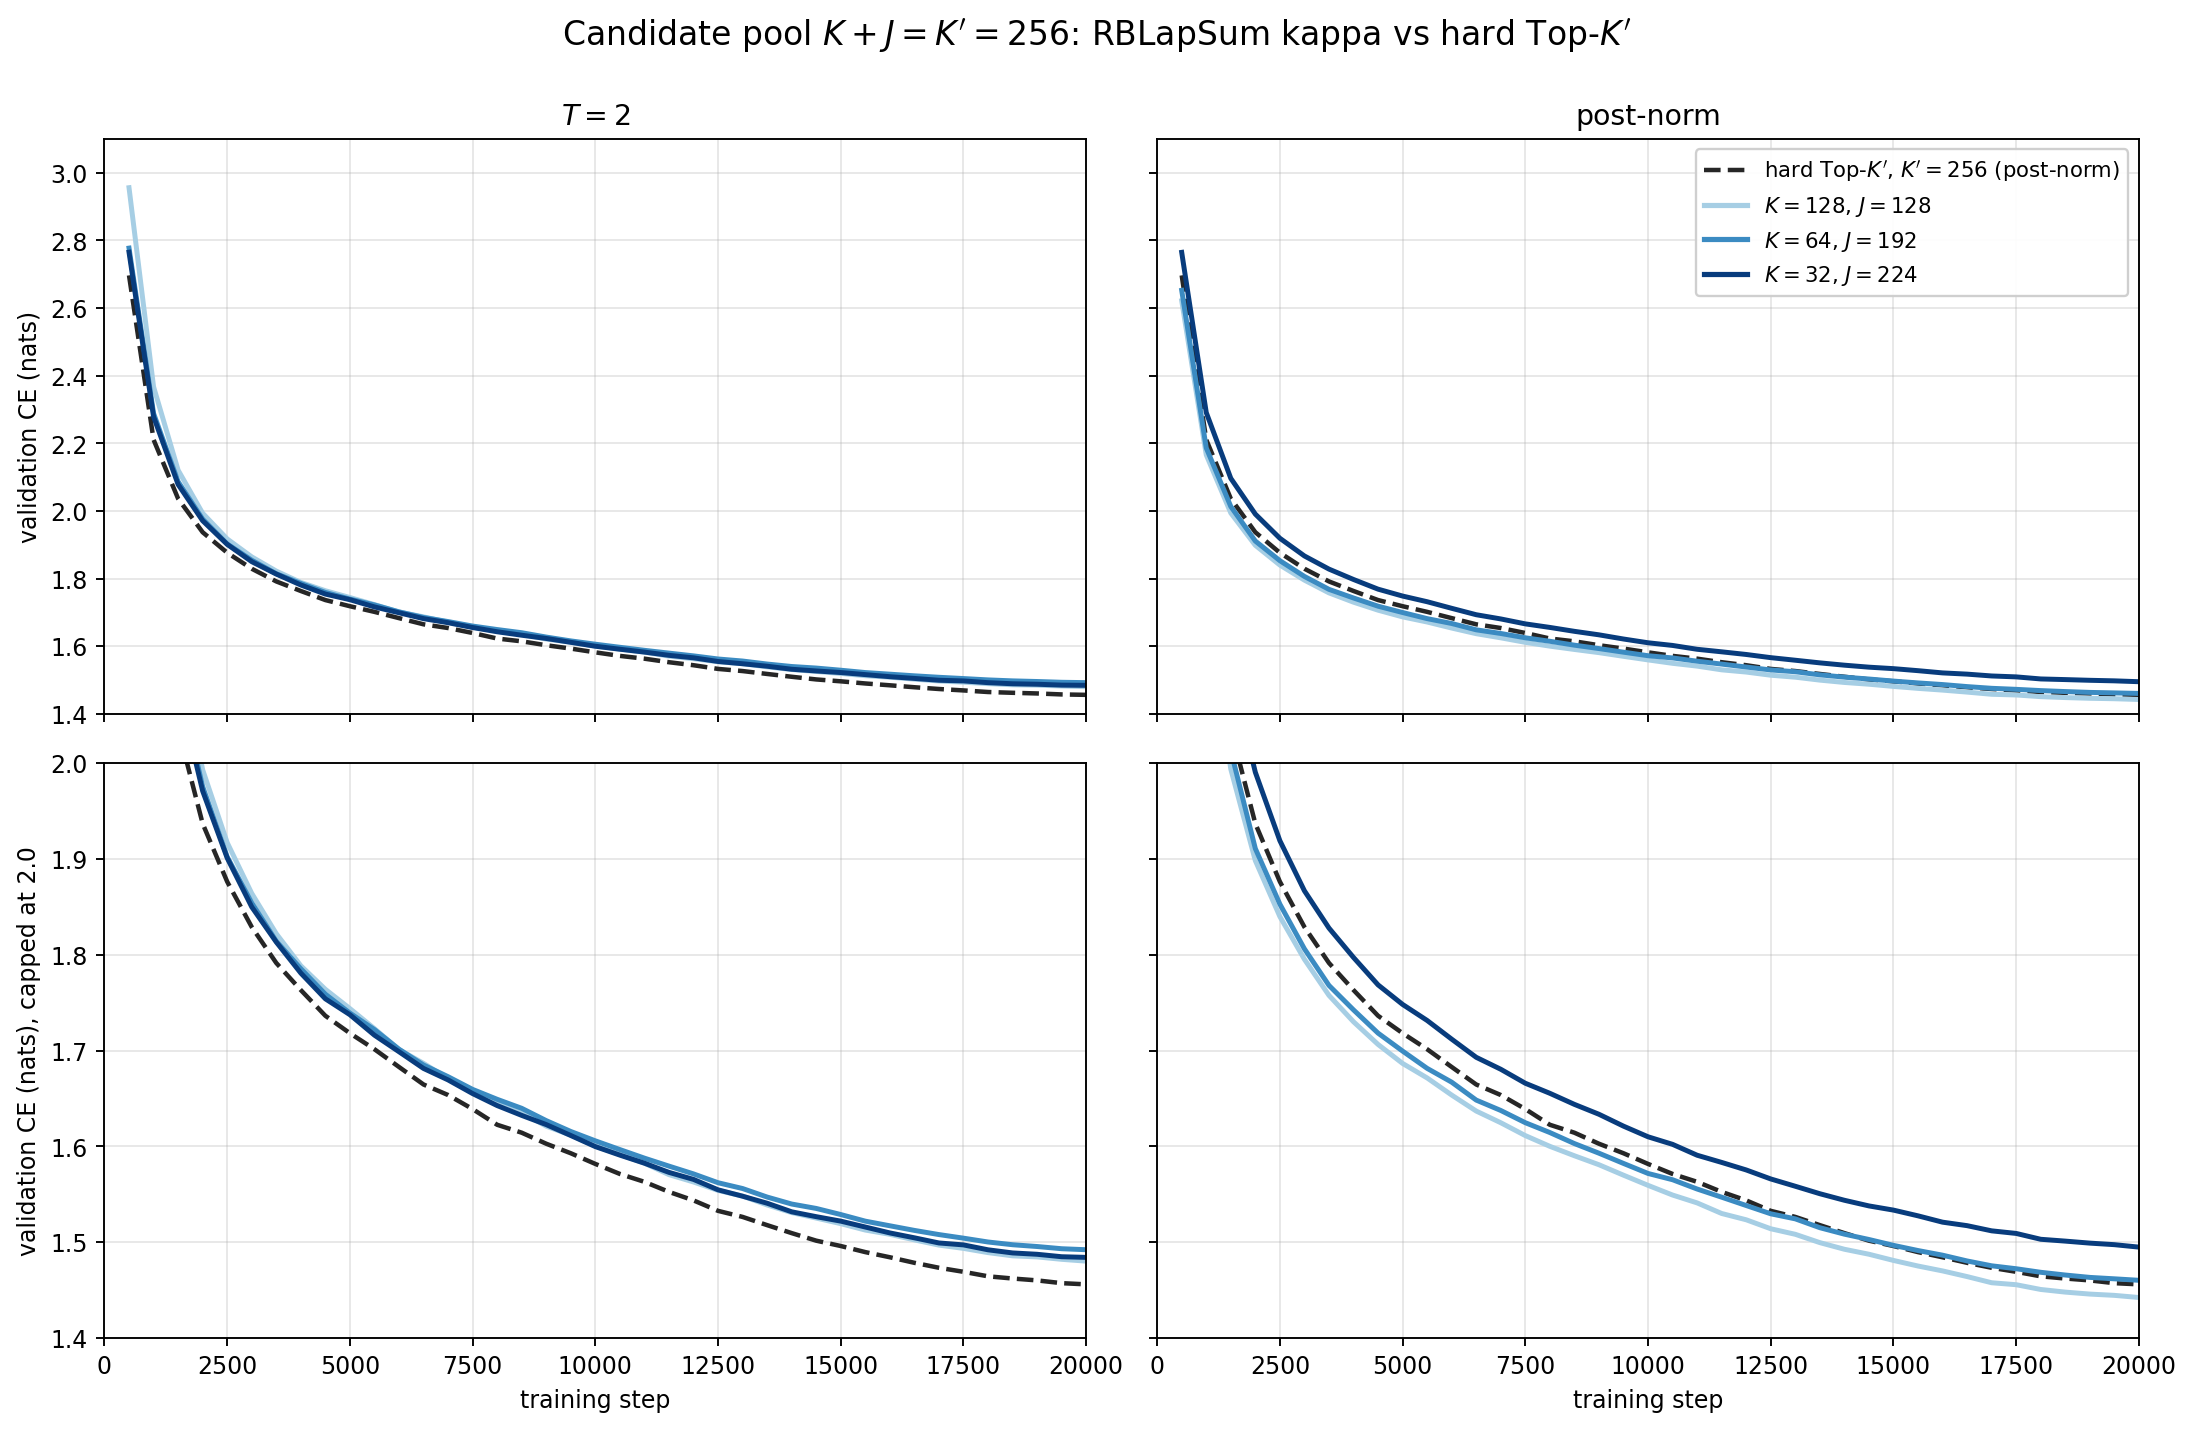
\includegraphics[width=\textwidth]{figures/kj_pool_k256.png}
\caption{$\Kp = 256$. Under the post-norm the $K=128$ curve separates from
the hard baseline from about step 5000 and stays below it; $K=64$ converges to
within $0.004$ nats of hard, and $K=32$ remains clearly above. At $T=2$ all
three sit above the baseline throughout.}
\end{figure}

\begin{figure}[p]\centering
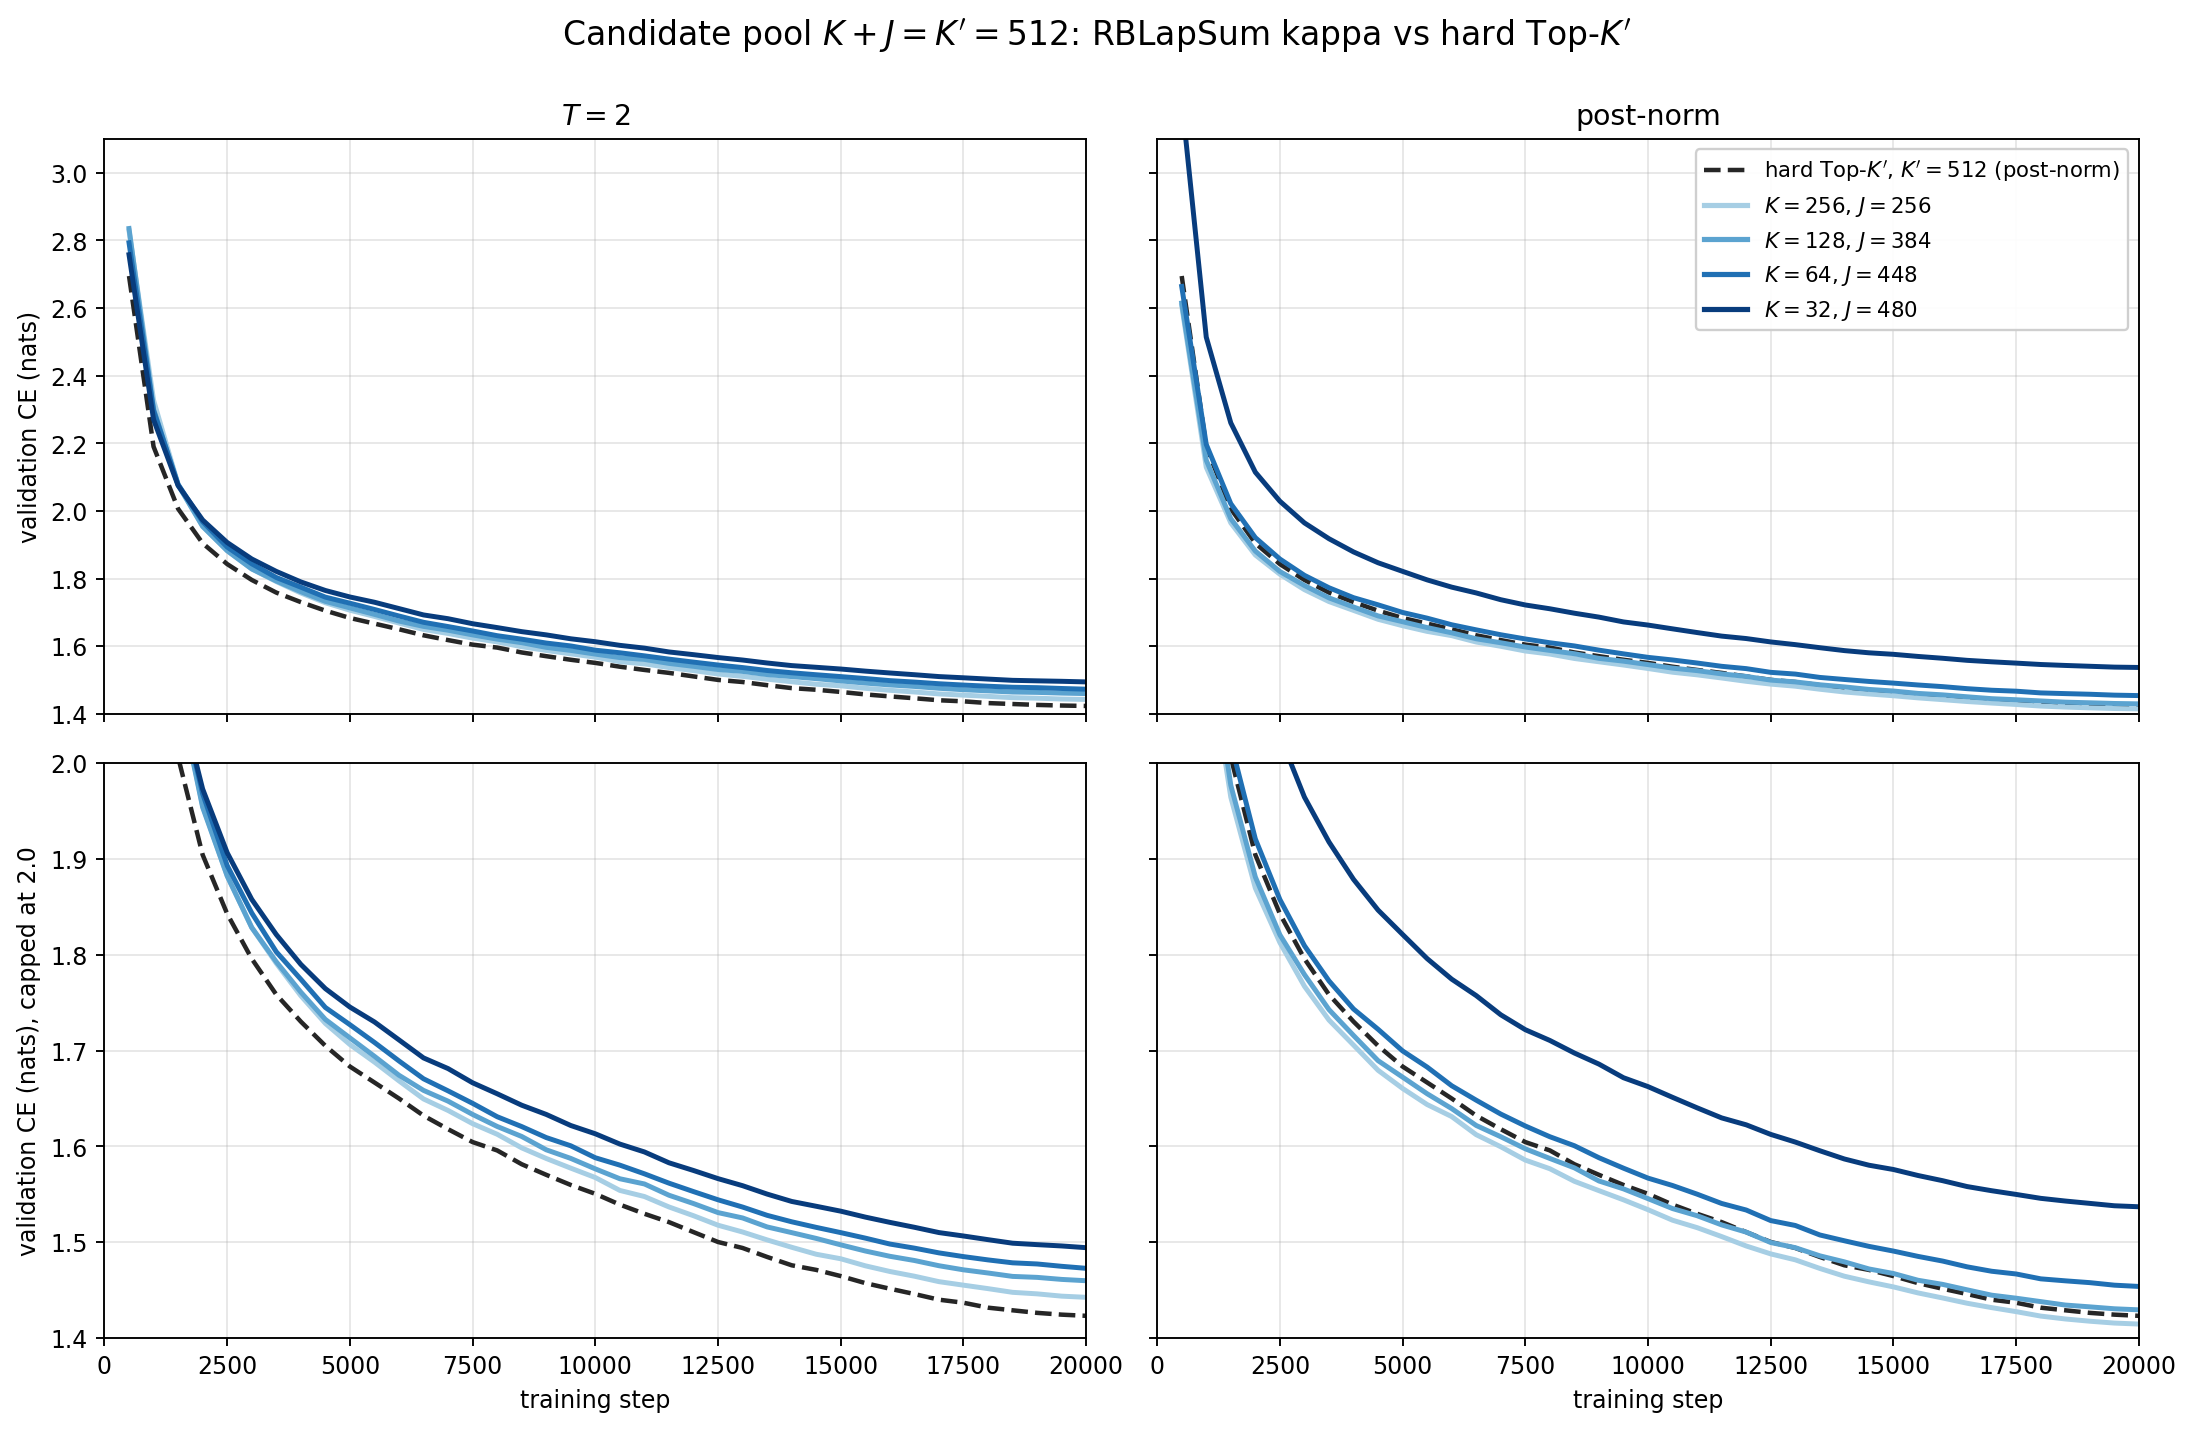
\includegraphics[width=\textwidth]{figures/kj_pool_k512.png}
\caption{$\Kp = 512$. The ordering is monotone in $K$: $K=256$ ends below
hard Top-512, $K=128$ tracks it to within $0.006$ nats, and $K=64$ and $K=32$
fall progressively behind. The $K=32$ curve is the reversal discussed above.}
\end{figure}

\clearpage
\subsection*{Per active count}

Each figure fixes the active count $K$ and shows every candidate window
trained at that $K$ (solid, a blue ramp light to dark with increasing $J$)
against all five hard Top-$\Kp$ baselines (dashed, a red ramp light to dark
with increasing $\Kp$). Hue separates the two families and lightness orders
each, so a surrogate curve is never confusable with a hard one. The hard
curves are identical in all four figures, so they serve as a fixed reference
scale.

\begin{figure}[p]\centering
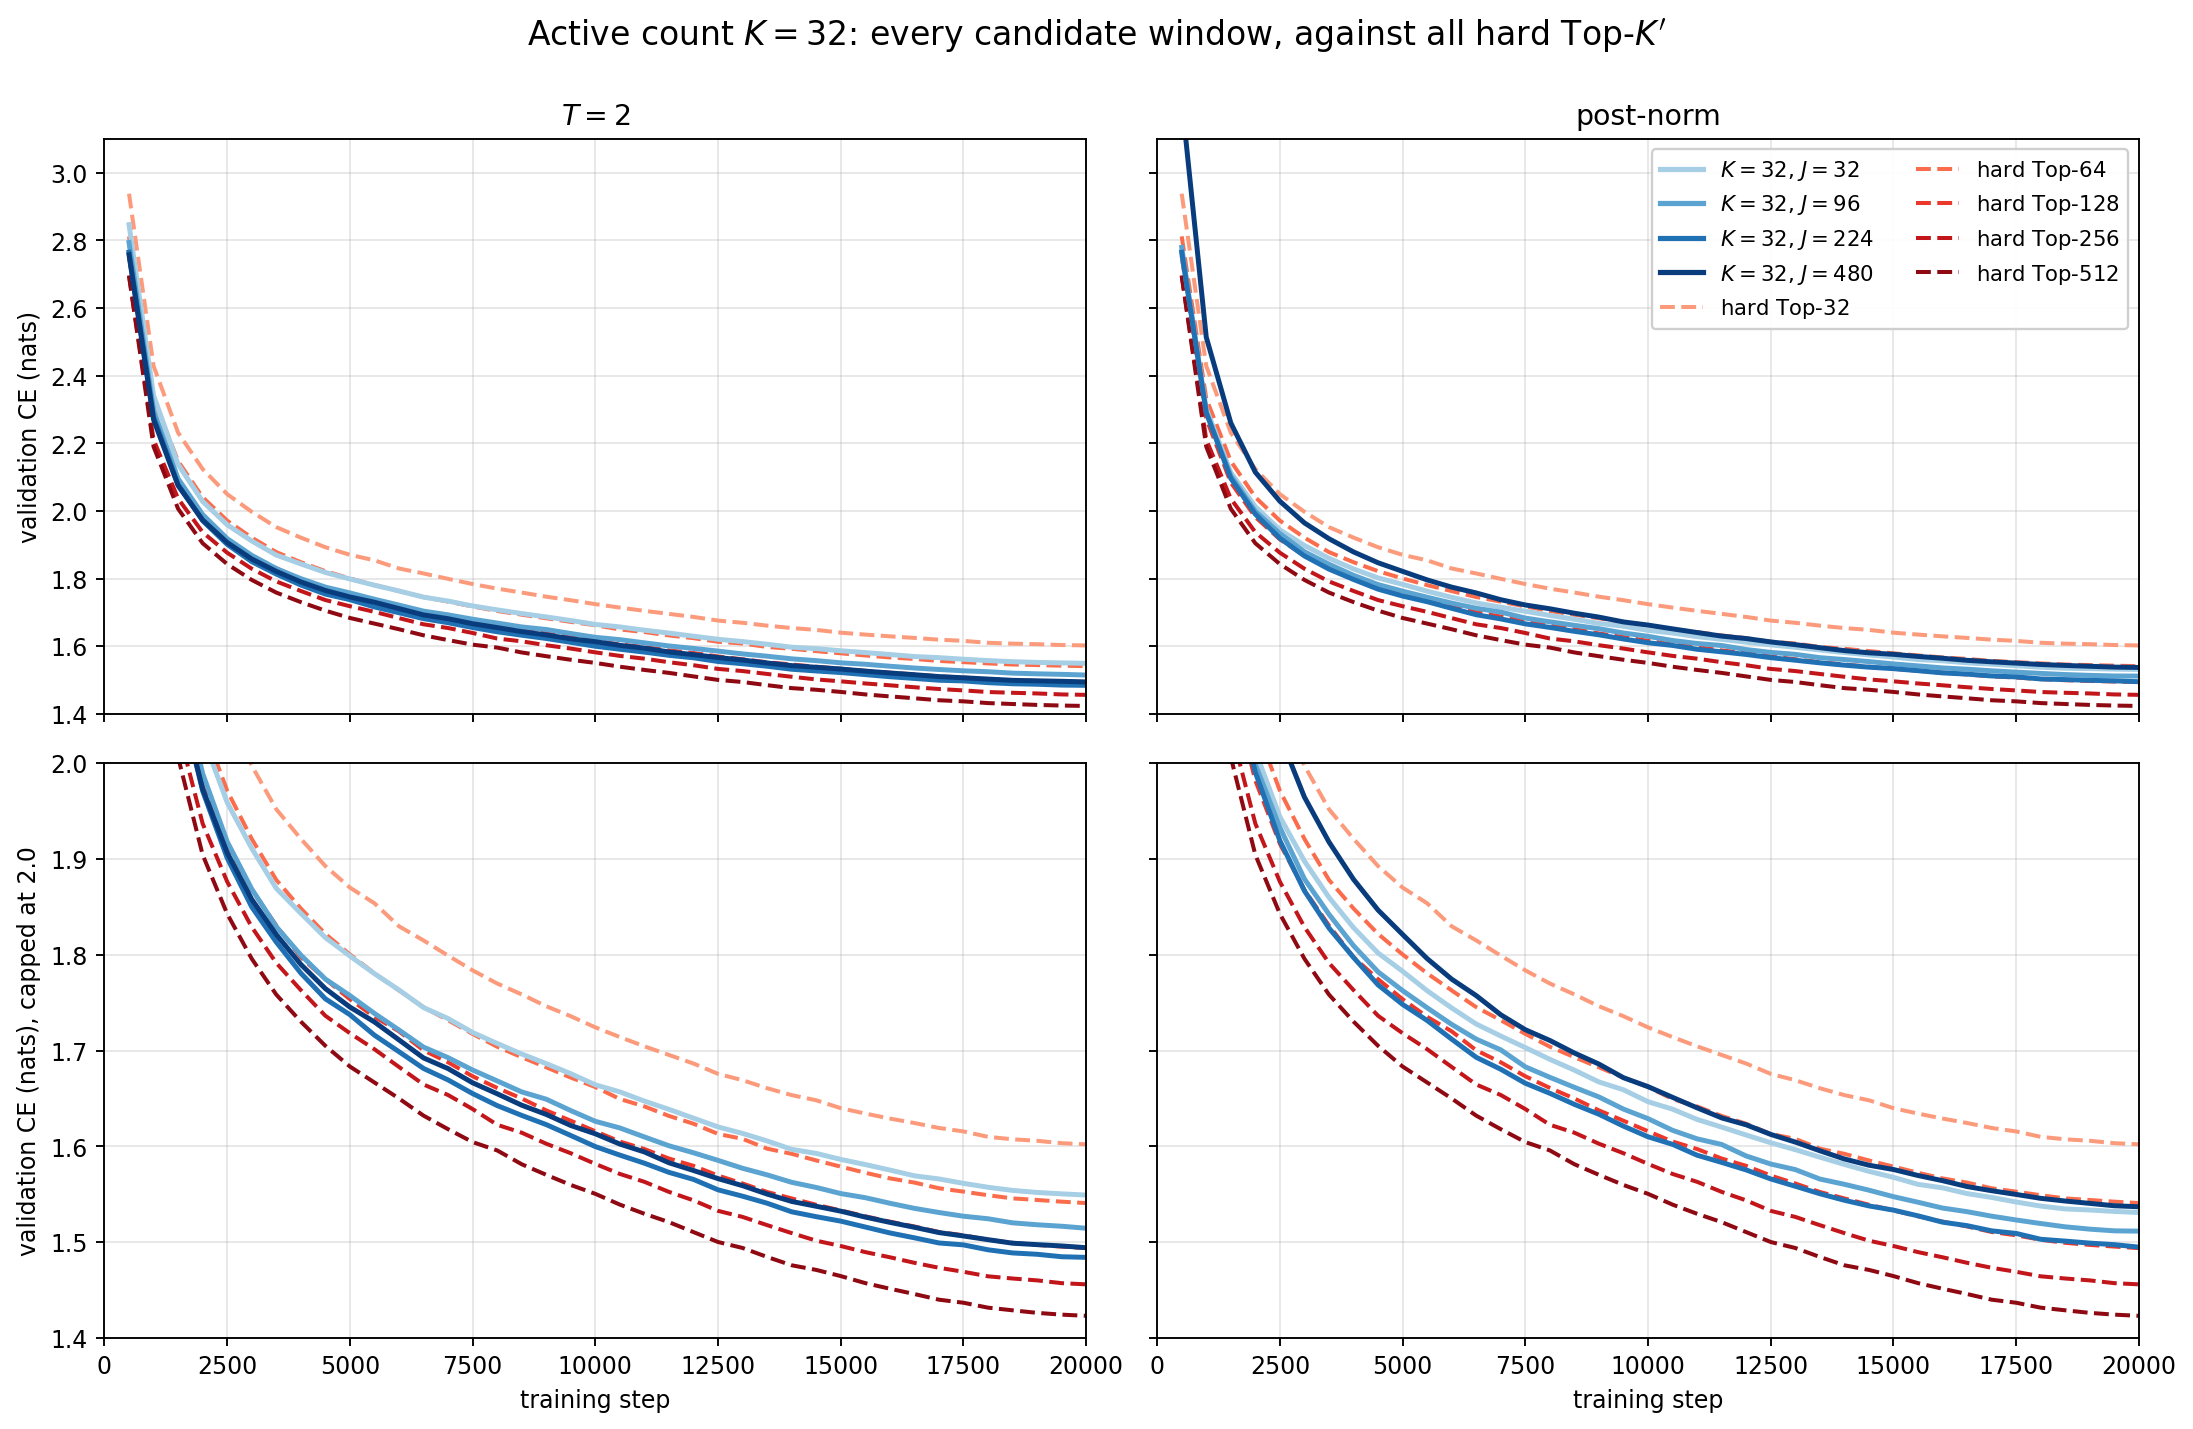
\includegraphics[width=\textwidth]{figures/kj_active_k32.png}
\caption{$K=32$. Widening the window moves the model up the hard ladder --
from between hard Top-32 and Top-64 at $J=32$ to past hard Top-128 at
$J=224$ -- but the widest window, $J=480$, falls back under the post-norm
while continuing to improve at $T=2$.}
\end{figure}

\begin{figure}[p]\centering
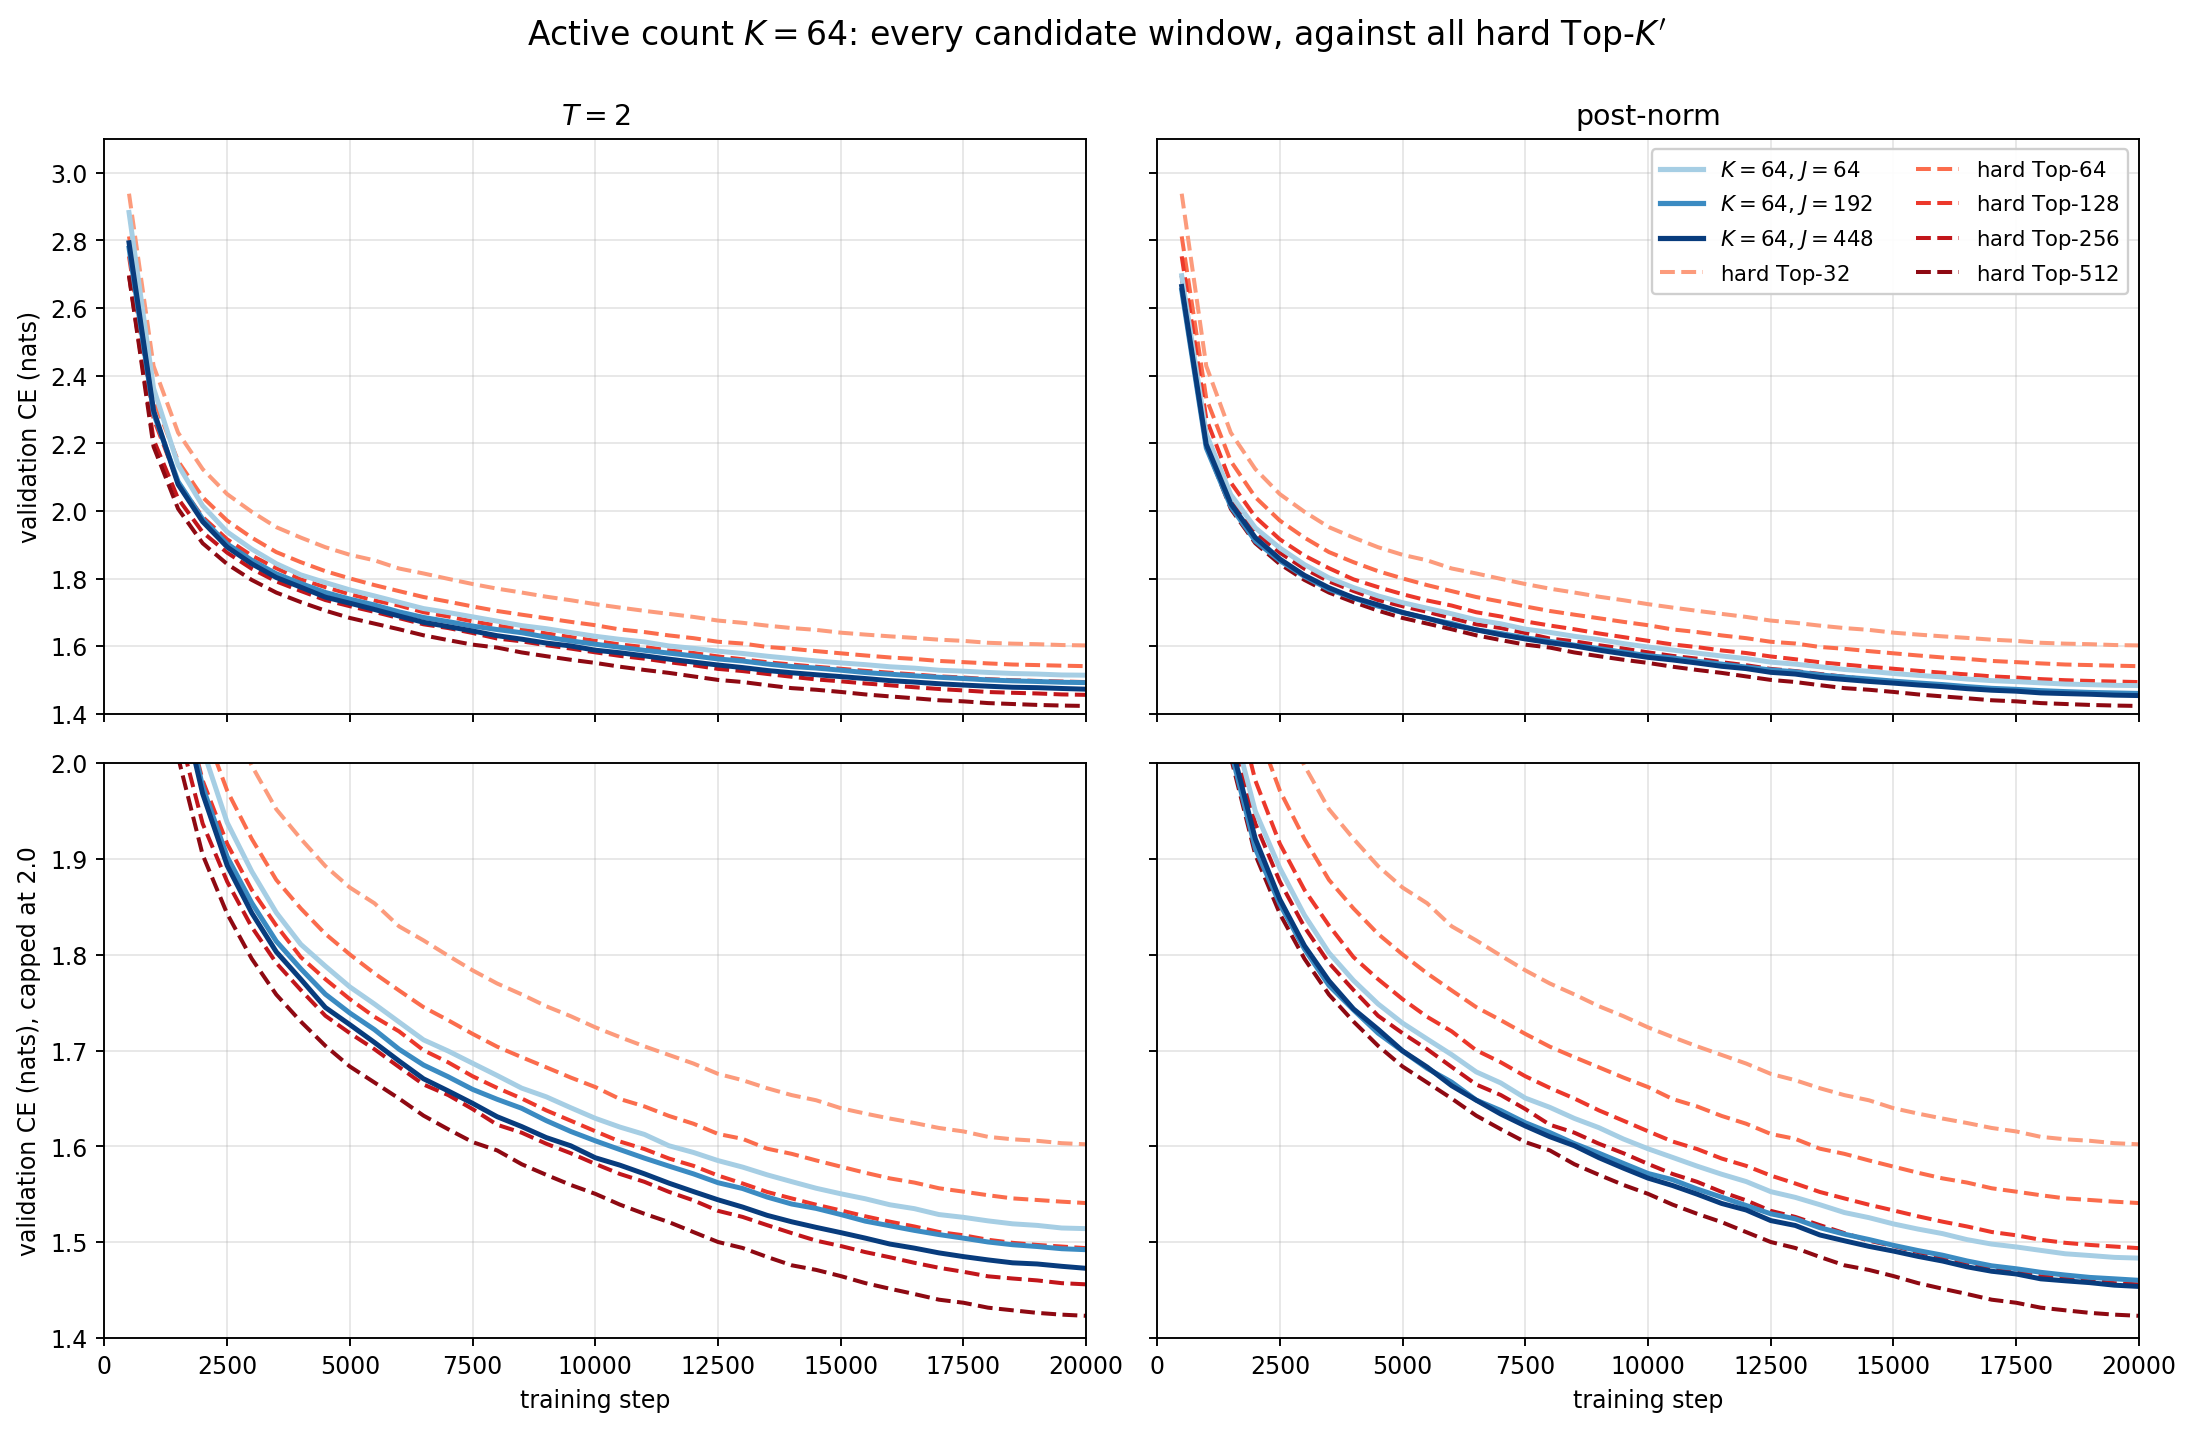
\includegraphics[width=\textwidth]{figures/kj_active_k64.png}
\caption{$K=64$. Every window improves on the last, and the best
($J=448$) lands between hard Top-256 and hard Top-512 while activating
64 features.}
\end{figure}

\begin{figure}[p]\centering
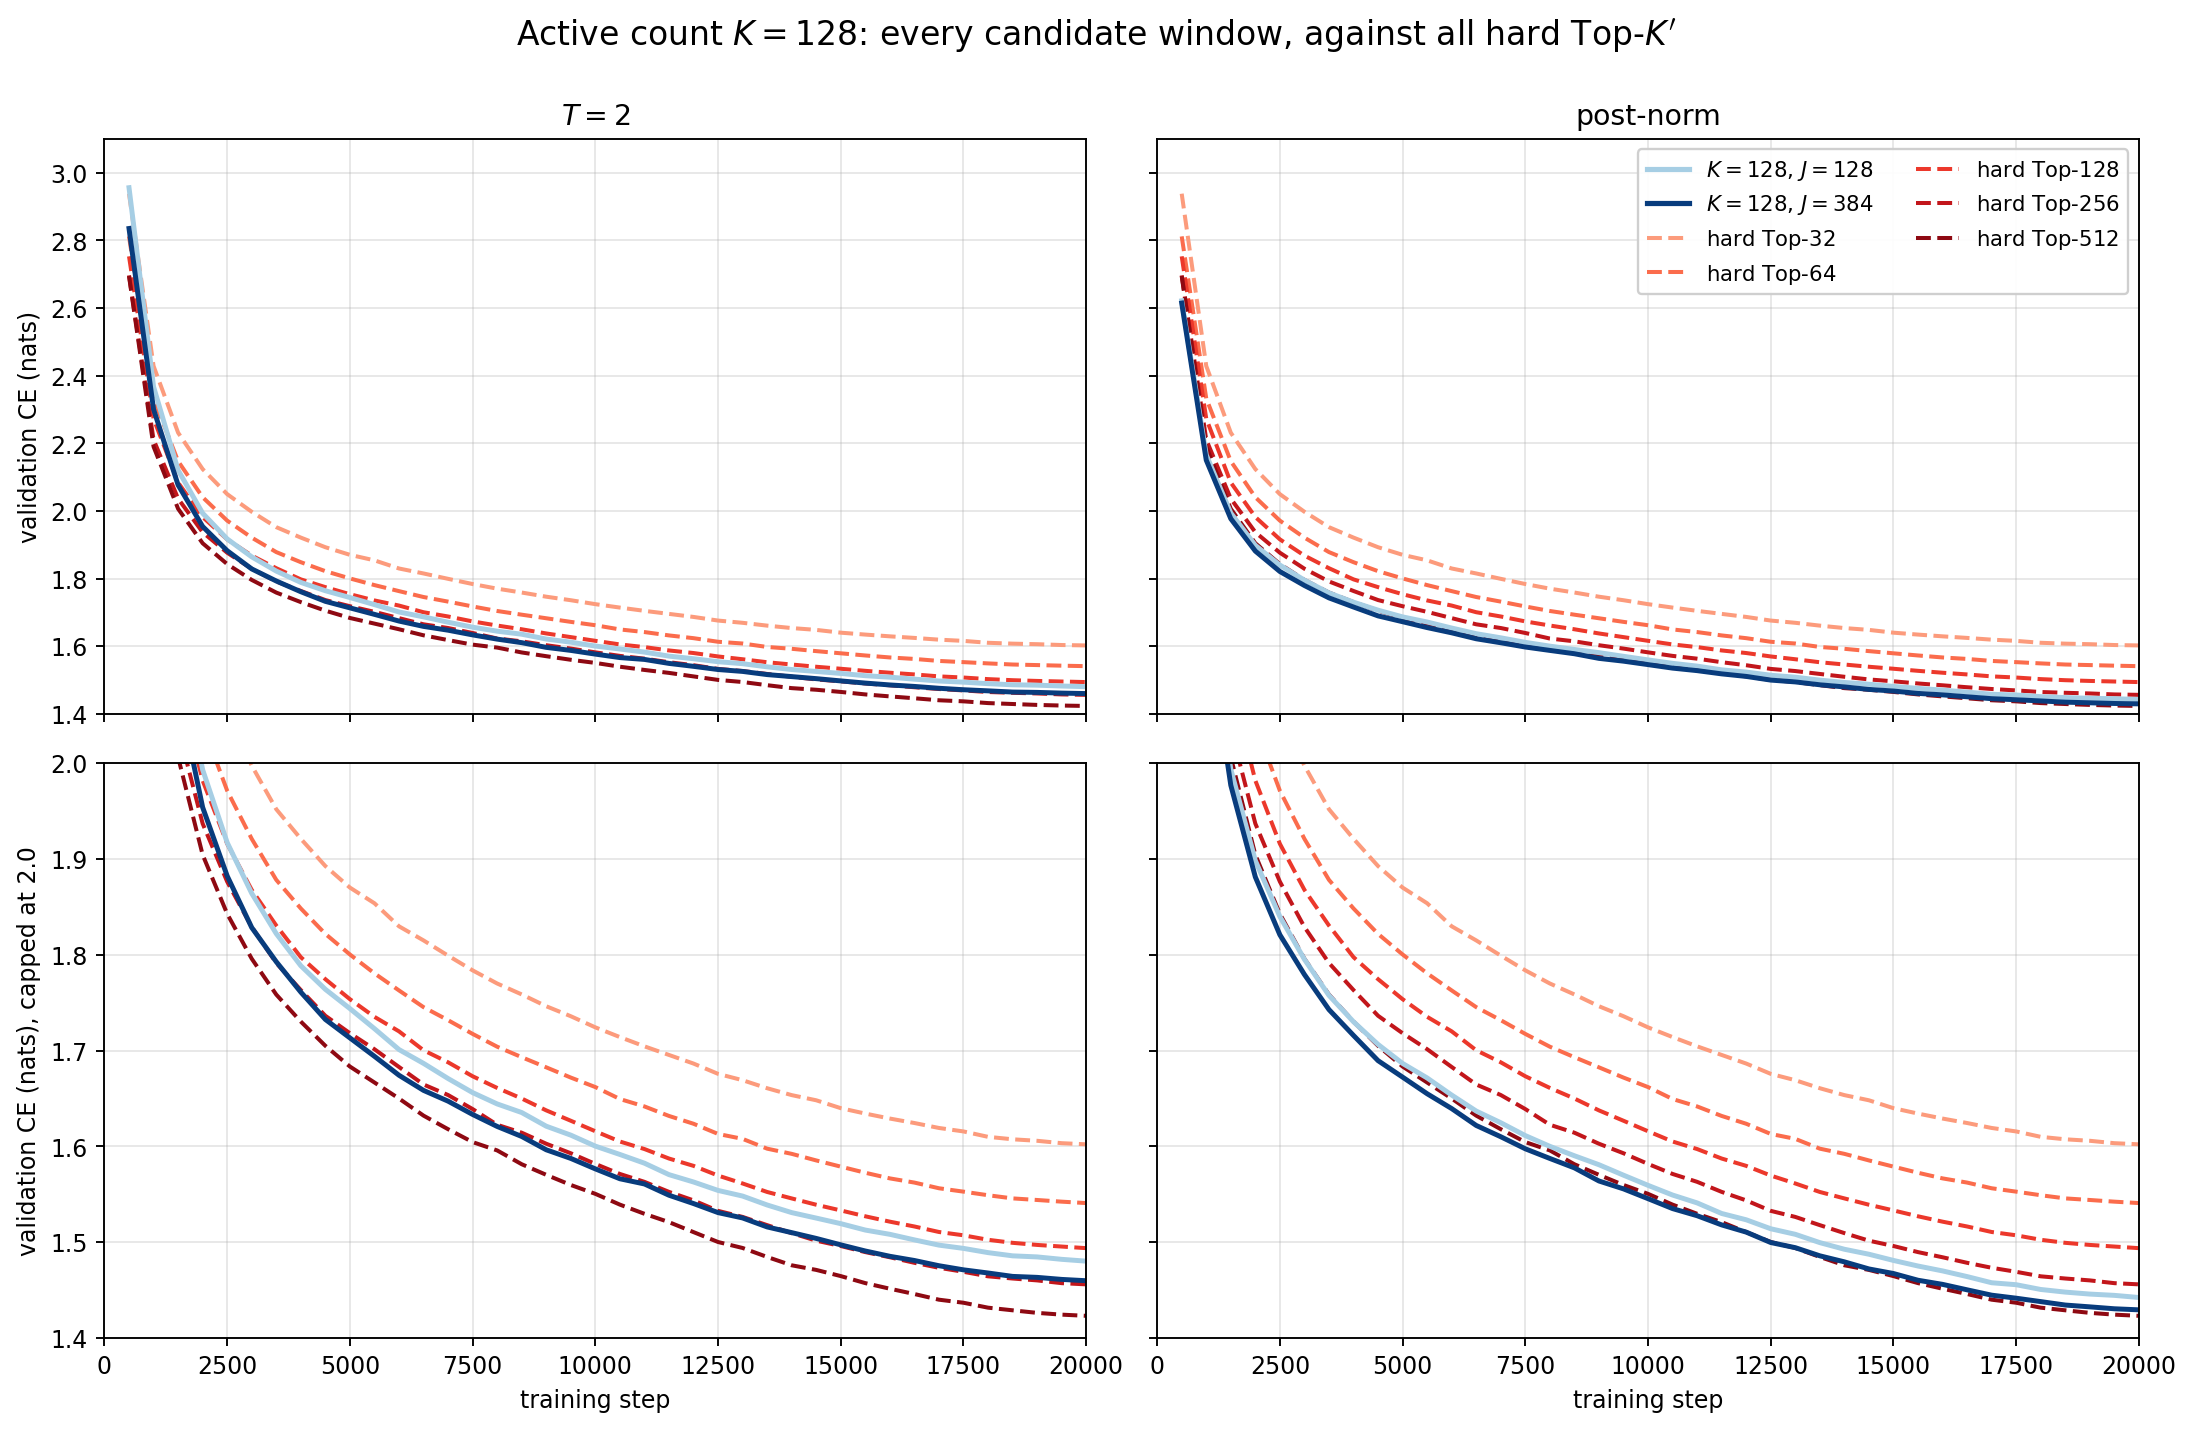
\includegraphics[width=\textwidth]{figures/kj_active_k128.png}
\caption{$K=128$. Both windows beat hard Top-256 under the post-norm, and
$J=384$ reaches hard Top-512 to within $0.006$ nats at a quarter of its
active count.}
\end{figure}

\begin{figure}[p]\centering
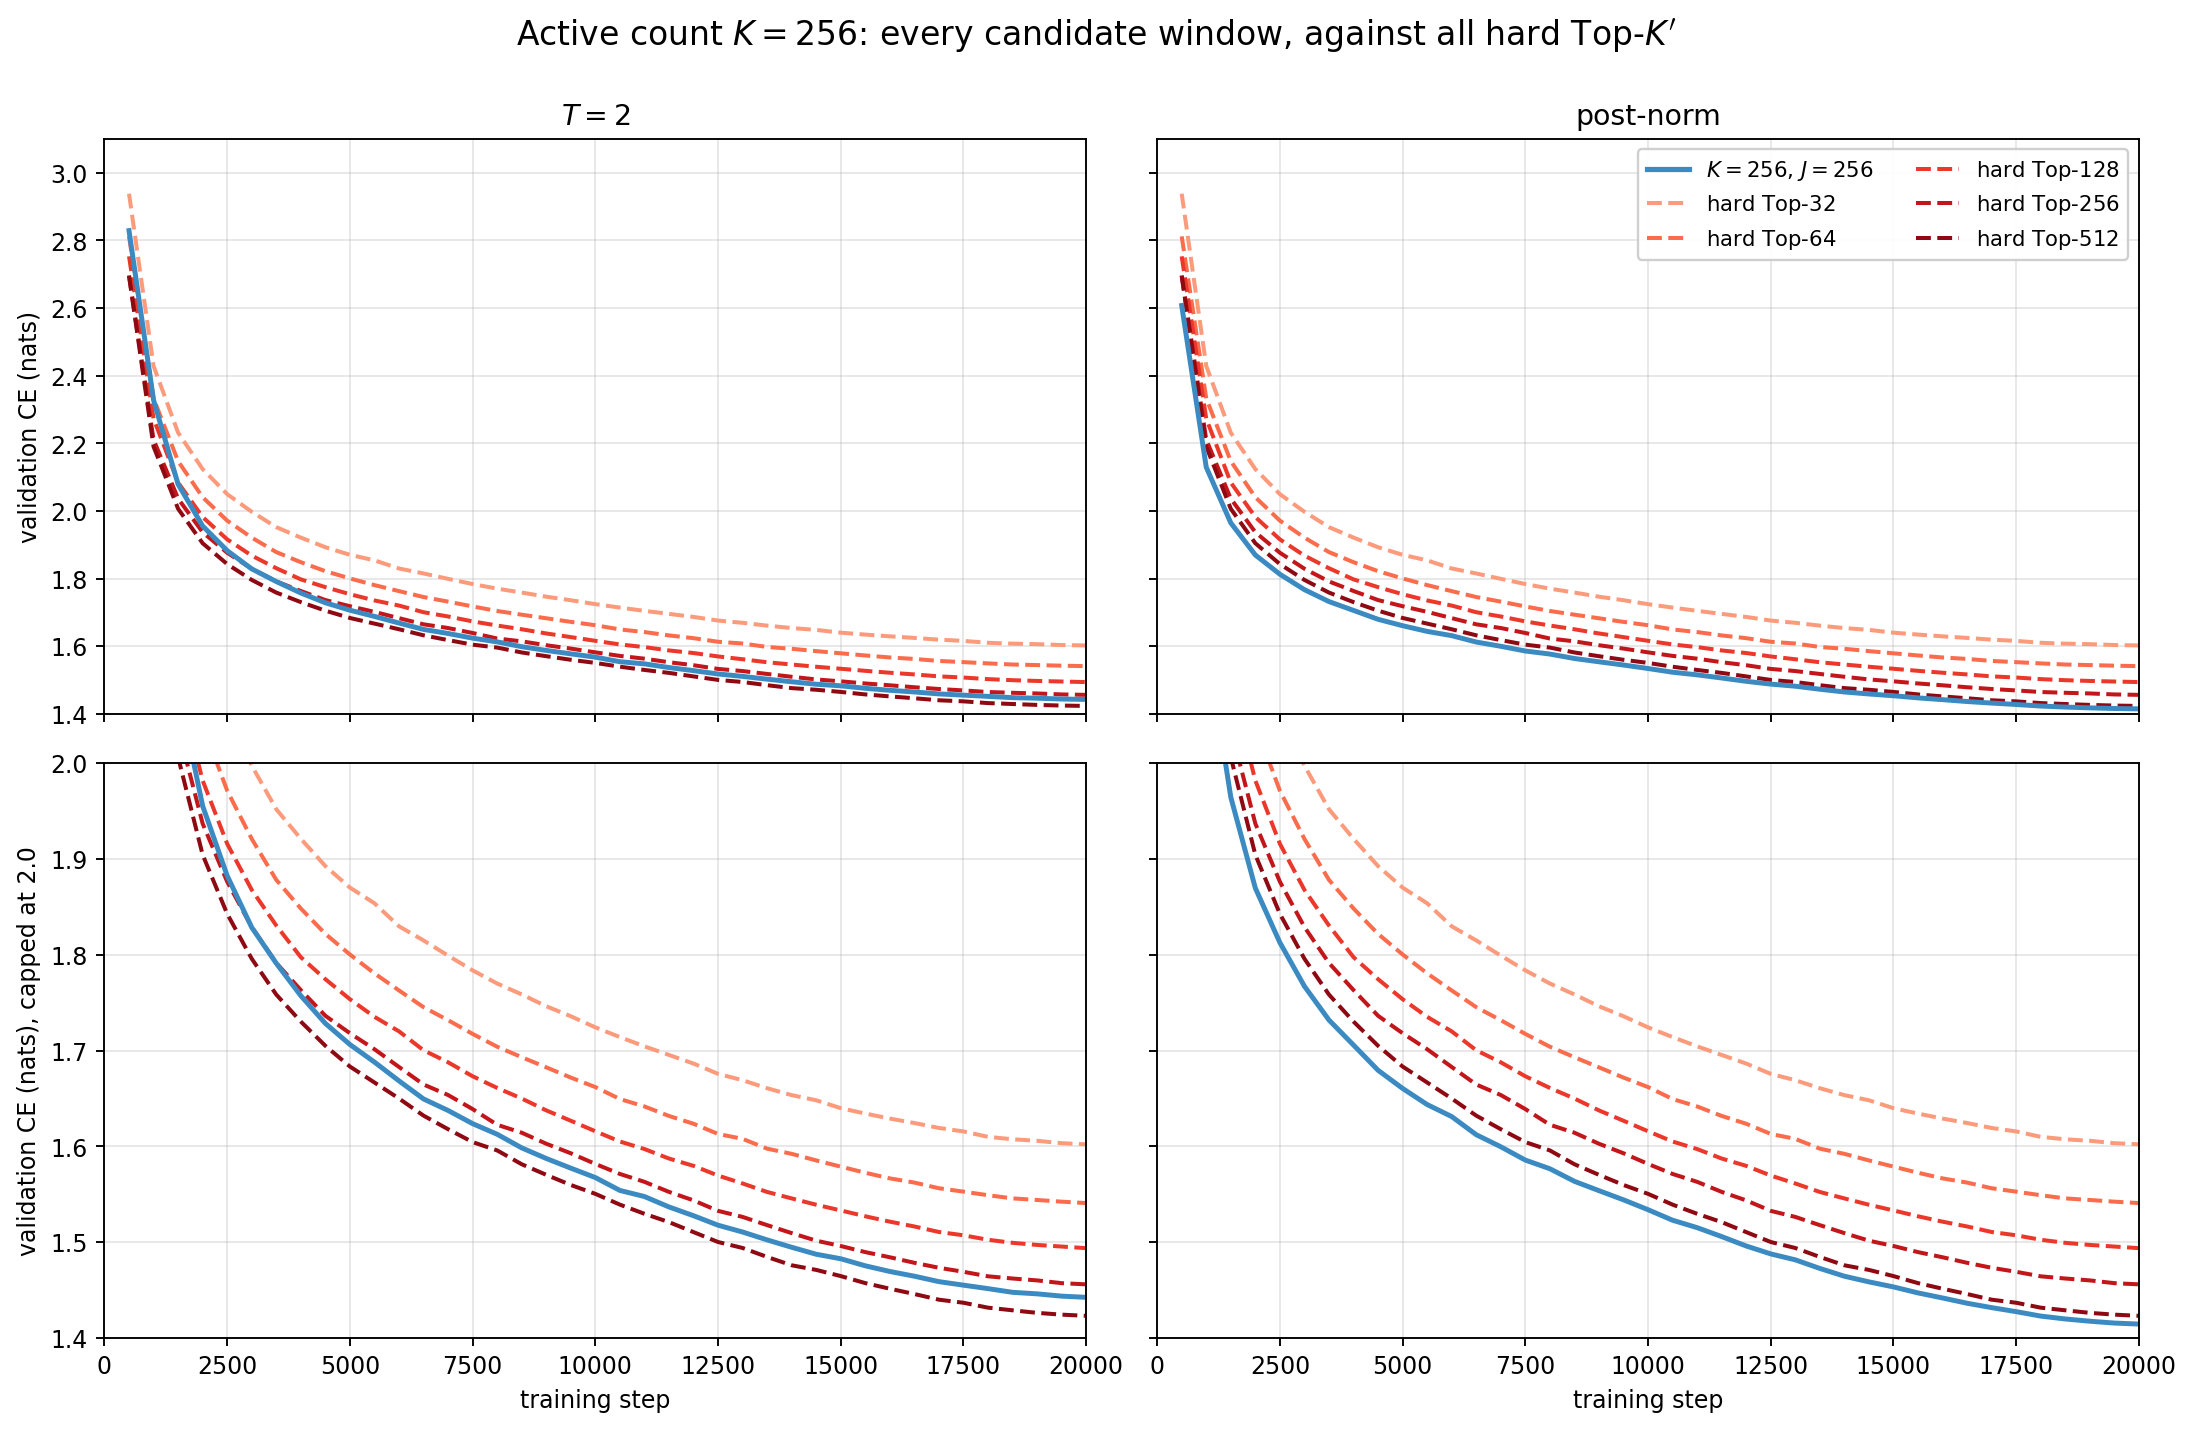
\includegraphics[width=\textwidth]{figures/kj_active_k256.png}
\caption{$K=256$. Under the post-norm the single cell ($J=256$) ends below
every hard baseline including Top-512, which is the best result in the
comparison. At $T=2$ the same cell sits between hard Top-256 and Top-512.}
\end{figure}

\clearpage

% ============================================================
\section{Interpretation}
% ============================================================

Two regularities organize the tables.

First, \textbf{the candidate window substitutes for active features, at a
roughly fixed exchange rate of about a factor of two}. Under the post-norm,
$K$ active features with a pool of $2K$ beat $2K$ active features with no
surrogate, and they do so at all four scales tested, with a margin
($0.009$--$0.014$ nats) that is remarkably stable across a factor of eight in
$K$. Pushing further -- a pool of $4K$ or more -- keeps improving the loss at
fixed $K$ but no longer beats the correspondingly larger hard model: at
$\Kp = 512$, $K=128$ (pool $4K$) lands $0.006$ nats short of hard Top-512
and $K=64$ (pool $8K$) $0.031$ short. The surrogate closes roughly one
doubling of the active count, not an unbounded amount.

Second, \textbf{the post-norm is the better variant almost everywhere, and
the exceptions need both a small active count and a very wide window}. It
wins 8 of the 10 cells, by $0.003$--$0.038$ nats; the two losses are $K=32$
with $J=224$ and $J=480$, where $T=2$ is ahead by $0.011$ and $0.043$. The
ratio alone does not explain it: $K=64$ with $J=448$ has the same $J/K = 7$
as the first loss and still favours the post-norm by $0.019$. What the two
exceptions share is a small support inside a window seven to fifteen times
wider -- the regime where the kernel must span far more candidates than the
model keeps, and where widening the kernel is the effective remedy while
normalizing the output is not. This is a sharpening of the stabilization
note's observation that the better variant was configuration-dependent, but
it remains an observation about two cells and not a mechanism.

Together the two regularities suggest a practical default: a pool of about
$2K$ with the output norm, and $T=2$ instead if the window must be much
wider than the support.

% ============================================================
\section{Scope}
% ============================================================

All cells are single runs at one seed. The differences that carry the
conclusions are of two sizes: the matched-active-count margins
($0.04$--$0.11$ nats) are large relative to anything seen from run-to-run
variation in this project, while the diagonal wins over hard Top-$\Kp$
($0.009$--$0.014$ nats) are small, and rest on their consistency across four
independent pools rather than on any single comparison. A seed repeat of the
four diagonal cells and their hard baselines would settle that directly.

The hard baselines all carry the post-norm, which the previous note measured
as a small improvement for hard bottlenecks ($-0.014$ at $K=32$, $-0.007$ at
$K=512$); against hard baselines without it the surrogate's margins would be
slightly larger. Only two variants were tested, and only one value of each
($T=2$; RMSNorm at $T=1$). Finally, $K+J \leq 512$ throughout, well inside
$N=1536$, so nothing here speaks to pools approaching the full feature set.

\end{document}
